\documentclass{beamer}
\usetheme{CambridgeUS}
\usefonttheme{professionalfonts}
\usepackage{times}
\usepackage{tikz}
\usepackage{amsmath}
\usepackage{verbatim}
\usepackage{graphicx}
\usepackage{hyperref}
\usetikzlibrary{arrows,shapes}

\author{Students of ISU}
\title{Implementing Euler's numerical method in Python}

\begin{document}
\begin{frame}{Stated problem}

  \begin{block}{Given: Differential Equation}
    \begin{eqnarray}
      f(t,T(t)) = \frac{dT}{dt}=-k(T(t)-T_{env}); \\
      \label{du}
      t_0=0, \quad T(t_0)=T_0.
    \end{eqnarray}
  \end{block}

  \begin{block}{Find:}
    \[
      T(t),\quad t>=t_0.
    \]
  \end{block}
\end{frame}
\begin{frame}{Euler's method of numerical integration}
  \begin{eqnarray}
    \Delta x = h = 0.001\;\; s,\\
    t_i = t_0 + nh, \\
    dT(t) = f(t,T(t))dt.\\
    \Delta T (t_{i+1}) = f(t_i,T(t_i))\cdot h,\\
    T(0)=T_{env},\quad t_0=0.
  \end{eqnarray}
\end{frame}

\begin{frame}{Result of the modeling}
  \begin{center}
  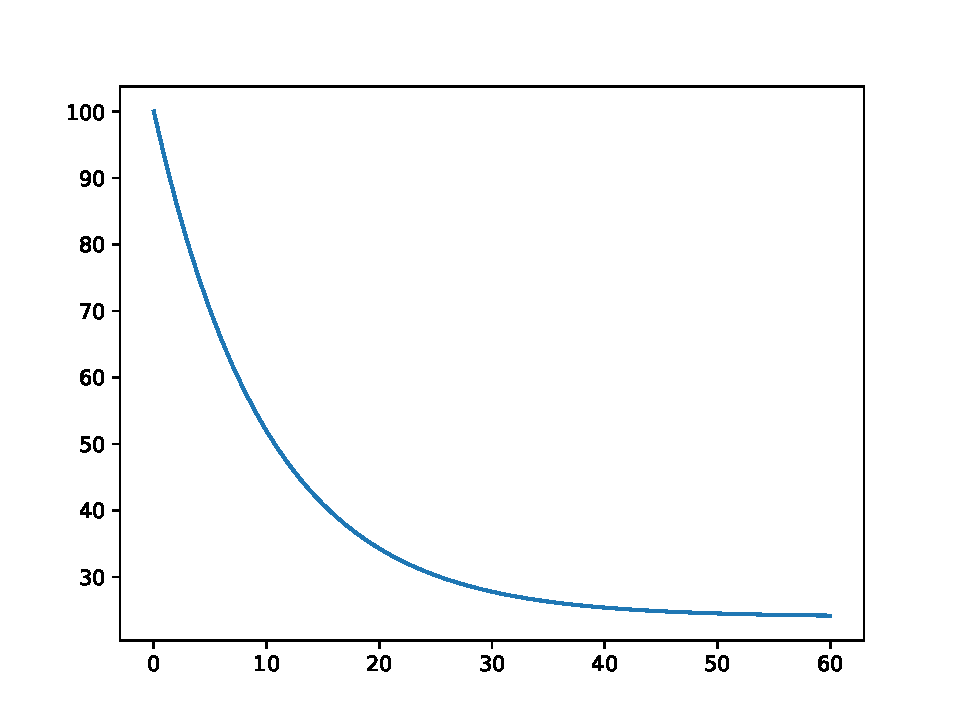
\includegraphics[width=0.8\linewidth]{trajectory.pdf}
\end{center}
\end{frame}
\begin{frame}{Conclusion}
  \url{http://edu.irnok.net/doku.php?id=euler:start}
\end{frame}


\end{document}







%%% Local Variables:
%%% mode: latex
%%% TeX-master: t
%%% End:
